
\documentclass[conference]{IEEEtran}
% Some Computer Society conferences also require the compsoc mode option,
% but others use the standard conference format.
%
% If IEEEtran.cls has not been installed into the LaTeX system files,
% manually specify the path to it like:
% \documentclass[conference]{../sty/IEEEtran}





% Some very useful LaTeX packages include:
% (uncomment the ones you want to load)


% *** CITATION PACKAGES ***
%
%\usepackage{cite}
% cite.sty was written by Donald Arseneau
% V1.6 and later of IEEEtran pre-defines the format of the cite.sty package
% \cite{} output to follow that of the IEEE. Loading the cite package will
% result in citation numbers being automatically sorted and properly
% "compressed/ranged". e.g., [1], [9], [2], [7], [5], [6] without using
% cite.sty will become [1], [2], [5]--[7], [9] using cite.sty. cite.sty's
% \cite will automatically add leading space, if needed. Use cite.sty's
% noadjust option (cite.sty V3.8 and later) if you want to turn this off
% such as if a citation ever needs to be enclosed in parenthesis.
% cite.sty is already installed on most LaTeX systems. Be sure and use
% version 5.0 (2009-03-20) and later if using hyperref.sty.
% The latest version can be obtained at:
% http://www.ctan.org/pkg/cite
% The documentation is contained in the cite.sty file itself.






% *** GRAPHICS RELATED PACKAGES ***
%
\ifCLASSINFOpdf
  \usepackage[pdftex]{graphicx}
  % declare the path(s) where your graphic files are
  % \graphicspath{{../pdf/}{../jpeg/}}
  % and their extensions so you won't have to specify these with
  % every instance of \includegraphics
  % \DeclareGraphicsExtensions{.pdf,.jpeg,.png}
\else
  % or other class option (dvipsone, dvipdf, if not using dvips). graphicx
  % will default to the driver specified in the system graphics.cfg if no
  % driver is specified.
  % \usepackage[dvips]{graphicx}
  % declare the path(s) where your graphic files are
  % \graphicspath{{../eps/}}
  % and their extensions so you won't have to specify these with
  % every instance of \includegraphics
  % \DeclareGraphicsExtensions{.eps}
\fi


% *** MATH PACKAGES ***
%
\usepackage{amsmath}
% A popular package from the American Mathematical Society that provides
% many useful and powerful commands for dealing with mathematics.
%
% Note that the amsmath package sets \interdisplaylinepenalty to 10000
% thus preventing page breaks from occurring within multiline equations. Use:
%\interdisplaylinepenalty=2500
% after loading amsmath to restore such page breaks as IEEEtran.cls normally
% does. amsmath.sty is already installed on most LaTeX systems. The latest
% version and documentation can be obtained at:
% http://www.ctan.org/pkg/amsmath





% *** SPECIALIZED LIST PACKAGES ***
%
%\usepackage{algorithmic}
% algorithmic.sty was written by Peter Williams and Rogerio Brito.
% This package provides an algorithmic environment fo describing algorithms.
% You can use the algorithmic environment in-text or within a figure
% environment to provide for a floating algorithm. Do NOT use the algorithm
% floating environment provided by algorithm.sty (by the same authors) or
% algorithm2e.sty (by Christophe Fiorio) as the IEEE does not use dedicated
% algorithm float types and packages that provide these will not provide
% correct IEEE style captions. The latest version and documentation of
% algorithmic.sty can be obtained at:
% http://www.ctan.org/pkg/algorithms
% Also of interest may be the (relatively newer and more customizable)
% algorithmicx.sty package by Szasz Janos:
% http://www.ctan.org/pkg/algorithmicx




% *** ALIGNMENT PACKAGES ***
%
%\usepackage{array}
% Frank Mittelbach's and David Carlisle's array.sty patches and improves
% the standard LaTeX2e array and tabular environments to provide better
% appearance and additional user controls. As the default LaTeX2e table
% generation code is lacking to the point of almost being broken with
% respect to the quality of the end results, all users are strongly
% advised to use an enhanced (at the very least that provided by array.sty)
% set of table tools. array.sty is already installed on most systems. The
% latest version and documentation can be obtained at:
% http://www.ctan.org/pkg/array


% IEEEtran contains the IEEEeqnarray family of commands that can be used to
% generate multiline equations as well as matrices, tables, etc., of high
% quality.

% *** FLOAT PACKAGES ***
%
%\usepackage{fixltx2e}
% fixltx2e, the successor to the earlier fix2col.sty, was written by
% Frank Mittelbach and David Carlisle. This package corrects a few problems
% in the LaTeX2e kernel, the most notable of which is that in current
% LaTeX2e releases, the ordering of single and double column floats is not
% guaranteed to be preserved. Thus, an unpatched LaTeX2e can allow a
% single column figure to be placed prior to an earlier double column
% figure.
% Be aware that LaTeX2e kernels dated 2015 and later have fixltx2e.sty's
% corrections already built into the system in which case a warning will
% be issued if an attempt is made to load fixltx2e.sty as it is no longer
% needed.
% The latest version and documentation can be found at:
% http://www.ctan.org/pkg/fixltx2e


%\usepackage{stfloats}
% stfloats.sty was written by Sigitas Tolusis. This package gives LaTeX2e
% the ability to do double column floats at the bottom of the page as well
% as the top. (e.g., "\begin{figure*}[!b]" is not normally possible in
% LaTeX2e). It also provides a command:
%\fnbelowfloat
% to enable the placement of footnotes below bottom floats (the standard
% LaTeX2e kernel puts them above bottom floats). This is an invasive package
% which rewrites many portions of the LaTeX2e float routines. It may not work
% with other packages that modify the LaTeX2e float routines. The latest
% version and documentation can be obtained at:
% http://www.ctan.org/pkg/stfloats
% Do not use the stfloats baselinefloat ability as the IEEE does not allow
% \baselineskip to stretch. Authors submitting work to the IEEE should note
% that the IEEE rarely uses double column equations and that authors should try
% to avoid such use. Do not be tempted to use the cuted.sty or midfloat.sty
% packages (also by Sigitas Tolusis) as the IEEE does not format its papers in
% such ways.
% Do not attempt to use stfloats with fixltx2e as they are incompatible.
% Instead, use Morten Hogholm'a dblfloatfix which combines the features
% of both fixltx2e and stfloats:
%
% \usepackage{dblfloatfix}
% The latest version can be found at:
% http://www.ctan.org/pkg/dblfloatfix




% *** PDF, URL AND HYPERLINK PACKAGES ***
%
%\usepackage{url}
% url.sty was written by Donald Arseneau. It provides better support for
% handling and breaking URLs. url.sty is already installed on most LaTeX
% systems. The latest version and documentation can be obtained at:
% http://www.ctan.org/pkg/url
% Basically, \url{my_url_here}.




% *** Do not adjust lengths that control margins, column widths, etc. ***
% *** Do not use packages that alter fonts (such as pslatex).         ***
% There should be no need to do such things with IEEEtran.cls V1.6 and later.
% (Unless specifically asked to do so by the journal or conference you plan
% to submit to, of course. )


% correct bad hyphenation here
\hyphenation{op-tical net-works semi-conduc-tor}


\begin{document}
%
% paper title
% Titles are generally capitalized except for words such as a, an, and, as,
% at, but, by, for, in, nor, of, on, or, the, to and up, which are usually
% not capitalized unless they are the first or last word of the title.
% Linebreaks \\ can be used within to get better formatting as desired.
% Do not put math or special symbols in the title.
\title{Power Allocation and Relay Selection in
Amplify-and-Forward Relaying
}


% author names and affiliations
% use a multiple column layout for up to three different
% affiliations
\author{\IEEEauthorblockN{Prudhvi Porandla \quad Prof. Prasanna Chaporkar}
\IEEEauthorblockA{ Electrical Engineering\\
Indian Institute of Technology Bombay\\
}
}


% use for special paper notices
%\IEEEspecialpapernotice{(Invited Paper)}




% make the title area
\maketitle

% As a general rule, do not put math, special symbols or citations
% in the abstract
\begin{abstract}
	Multihop communication is considered to be a standard in next generation
	cellular networks.  There are several relaying schemes,
	Decode-and-forward(DF) and Amplify-and-Forward(AF) being the popular ones.
	In DF scheme, the relay decodes the message from the source, re- encodes
	and transmits it to the destination node whereas in AF the relay amplifies
	the received signal and transmits to the destination node. Relay selection
	and optimal power allocation are the two important aspects in either
	scheme. In this work, we look at these two problems in 2- hop communication
	network in which relays employ AF scheme. To make the power allocation
	problem well-defined we prove that rate/capacity is a concave function of
	both source and relay powers. Once concavity is established, we can find
	the optimal relay and source powers. However, when there are multiple
	relays the power allocation might interfere with relay selection. We show
	that this is indeed the case and discuss the conditions under which a relay
	switch over can take place.

\end{abstract}

% no keywords




% For peer review papers, you can put extra information on the cover page as
% needed: \ifCLASSOPTIONpeerreview \begin{center} \bfseries EDICS Category:
% 3-BBND \end{center} \fi
%
% For peerreview papers, this IEEEtran command inserts a page break and creates
% the second title. It will be ignored for other modes.
\IEEEpeerreviewmaketitle



\section{Introduction}
% no \IEEEPARstart
This demo file is intended to serve as a ``starter file'' for IEEE conference
papers produced under \LaTeX\ using IEEEtran.cls version 1.8b and later.
% You must have at least 2 lines in the paragraph with the drop letter (should
% never be an issue)
I wish you the best of success.

\hfill mds

\hfill August 26, 2015

\subsection{Subsection Heading Here} Subsection text here.


\subsubsection{Subsubsection Heading Here} Subsubsection text here.


% An example of a floating figure using the graphicx package.  Note that \label
% must occur AFTER (or within) \caption.  For figures, \caption should occur
% after the \includegraphics.  Note that IEEEtran v1.7 and later has special
% internal code that is designed to preserve the operation of \label within
% \caption even when the captionsoff option is in effect. However, because of
% issues like this, it may be the safest practice to put all your \label just
% after \caption rather than within \caption{}.
%
% Reminder: the "draftcls" or "draftclsnofoot", not "draft", class option
% should be used if it is desired that the figures are to be displayed while in
% draft mode.
%
%\begin{figure}[!t] \centering \includegraphics[width=2.5in]{myfigure} where an
%.eps filename suffix will be assumed under latex, and a .pdf suffix will be
%assumed for pdflatex; or what has been declared via
%\DeclareGraphicsExtensions.  \caption{Simulation results for the network.}
%\label{fig_sim} \end{figure}

% Note that the IEEE typically puts floats only at the top, even when this
% results in a large percentage of a column being occupied by floats.


% An example of a double column floating figure using two subfigures.  (The
% subfig.sty package must be loaded for this to work.) The subfigure \label
% commands are set within each subfloat command, and the \label for the overall
% figure must come after \caption.  \hfil is used as a separator to get equal
% spacing.  Watch out that the combined width of all the subfigures on a line
% do not exceed the text width or a line break will occur.
%
%\begin{figure*}[!t] \centering \subfloat[Case
%I]{\includegraphics[width=2.5in]{box}% \label{fig_first_case}} \hfil
%\subfloat[Case II]{\includegraphics[width=2.5in]{box}%
%\label{fig_second_case}} \caption{Simulation results for the network.}
%\label{fig_sim} \end{figure*}
%
% Note that often IEEE papers with subfigures do not employ subfigure captions
% (using the optional argument to \subfloat[]), but instead will
% reference/describe all of them (a), (b), etc., within the main caption.  Be
% aware that for subfig.sty to generate the (a), (b), etc., subfigure labels,
% the optional argument to \subfloat must be present. If a subcaption is not
% desired, just leave its contents blank, e.g., \subfloat[].


% An example of a floating table. Note that, for IEEE style tables, the
% \caption command should come BEFORE the table and, given that table captions
% serve much like titles, are usually capitalized except for words such as a,
% an, and, as, at, but, by, for, in, nor, of, on, or, the, to and up, which are
% usually not capitalized unless they are the first or last word of the
% caption. Table text will default to \footnotesize as the IEEE normally uses
% this smaller font for tables.  The \label must come after \caption as always.
%
%\begin{table}[!t]
%% increase table row spacing, adjust to taste
%\renewcommand{\arraystretch}{1.3} if using array.sty, it might be a good idea
%to tweak the value of \extrarowheight as needed to properly center the text
%within the cells \caption{An Example of a Table} \label{table_example}
%\centering
%% Some packages, such as MDW tools, offer better commands for making tables
%% than the plain LaTeX2e tabular which is used here.
%\begin{tabular}{|c||c|} \hline One & Two\\ \hline Three & Four\\ \hline
%\end{tabular} \end{table}


% Note that the IEEE does not put floats in the very first column
% - or typically anywhere on the first page for that matter. Also,
% in-text middle ("here") positioning is typically not used, but it is allowed
% and encouraged for Computer Society conferences (but not Computer Society
% journals). Most IEEE journals/conferences use top floats exclusively.  Note
% that, LaTeX2e, unlike IEEE journals/conferences, places footnotes above
% bottom floats. This can be corrected via the \fnbelowfloat command of the
% stfloats package.



\section{Amplify-and-Forward Relaying}
Consider 2-hop relaying; we have a source node, the destination, and a relay
node. In amplify-and-forward(AF) relaying scheme, the total transmission period is
divided in to two slots.
In the first slot, source node broadcasts the message to relay and destination nodes
and in the second the relay amplifies the received signal and retransmits it to 
the destination node. This is illustrated in fig~\ref{twoSlots}.
\begin{figure}[!t] 
	\centering 
	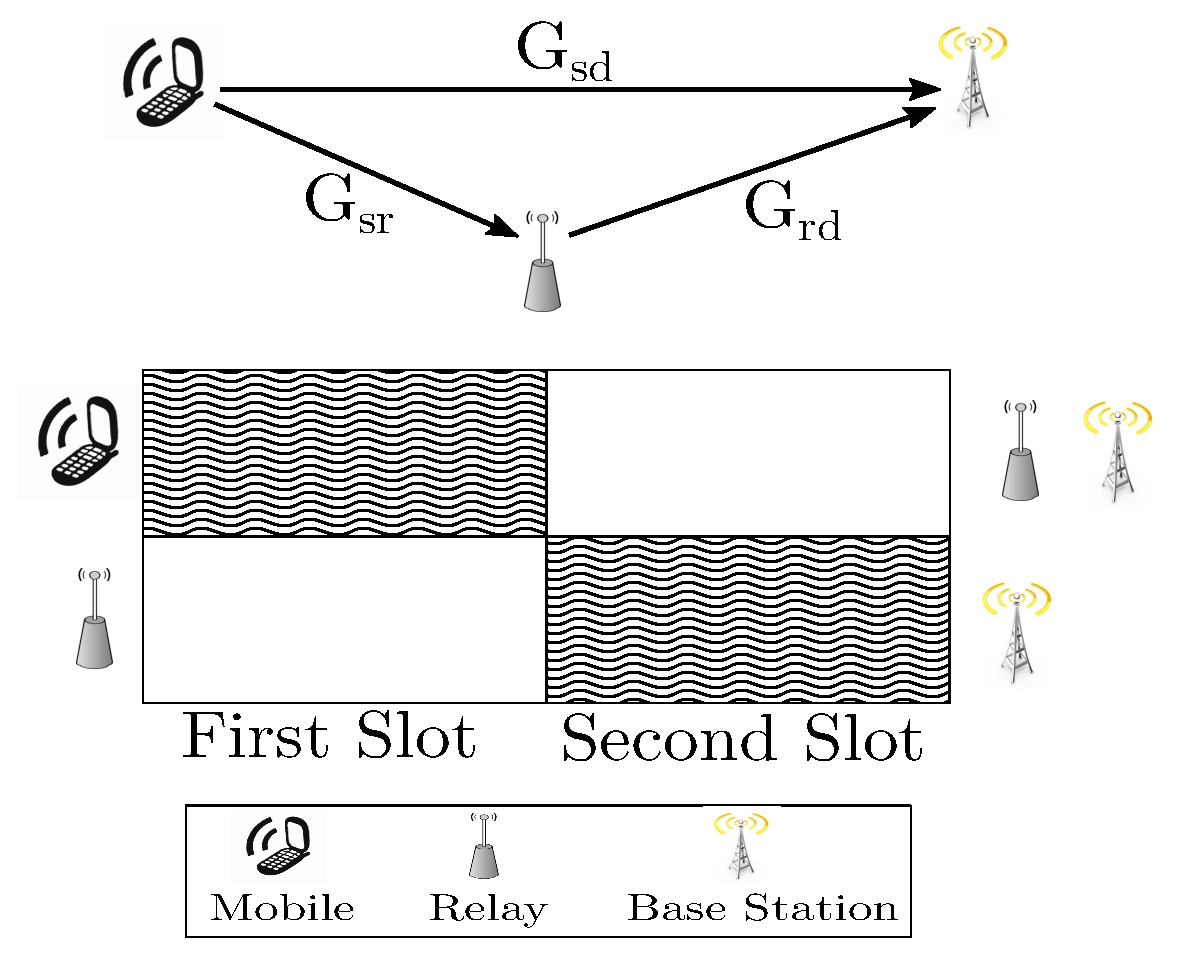
\includegraphics[width=2.5in]{img/sysmodel} 
	\caption{Two slots in AF}
	\label{twoSlots} 
\end{figure}
\subsection{Received Signals }
The signals received at relay and destination nodes in the two slots are as 
follows:\\
\textit{First Slot:}
\begin{align} \label{ysd}
	Y_{sd} &= \sqrt{P_s G_{sd}} X_s + n_{sd}
\end{align}
\begin{align*}
	Y_{sr} &= \sqrt{P_s G_{sr}} X_s + n_{sr} \\
\end{align*}
\textit{Second Slot:}
\begin{equation}\label{yrd}
	Y_{rd} = \sqrt{P_r G_{rd}} X_{rd} + n_{rd} 
\end{equation}
\begin{equation} \label{finalyrd}
	Y_{rd} = \frac{\sqrt{\mathstrut P_r G_{rd} P_s G_{sr}}}{\sqrt{\mathstrut 
	P_s G_{sr} + \sigma^2}}X_s + \frac{\sqrt{\mathstrut P_rG_{rd}}}{\sqrt{\mathstrut 
	P_s G_{sr} + \sigma^2}} n_{sr} + n_{rd} 
\end{equation}
The final expression for $Y_{rd}$ is obtained by substituting
$X_{rd} = \frac{Y_{sr}}{|Y_{sr}|}$ in eq.~\ref{yrd}. All symbols have usual
meanings - $s$ denotes source, $P$ denotes power, $G_{sd}\big(=\frac{g_{sd}}{\mathstrut
d^2_{sd}}\big)$ is the channel gain from source to destination, etc.
\subsection{Rate}
The rate/capacity of AF relaying scheme is given by
\begin{align*}
	R = \frac{1}{2} w \log_2(1+\Gamma_{sd}+\Gamma_{rd}) 
	\\ \text{where $\Gamma$
represents SNR}
\end{align*}
Substituting $\Gamma_{sd}$ and $\Gamma_{rd}$, obtained from equations \ref{ysd}
and \ref{finalyrd} respectively, in the above expression we get
\begin{align*}
	R &= \frac{1}{2} w \log_2\bigg(1+\frac{P_s G_{sd}}{\sigma^2} +
	\frac{P_s G_{sr} P_r G_{rd}}{\sigma^2(\sigma^2 + P_sG_{sr} + P_rG_{rd})}\bigg)
\end{align*}

\section{Source power and Relay selection}
\section{Future Work}
\section{Conclusion} The conclusion goes here.




% conference papers do not normally have an appendix




% trigger a \newpage just before the given reference number - used to balance
% the columns on the last page adjust value as needed - may need to be
% readjusted if the document is modified later
%\IEEEtriggeratref{8} The "triggered" command can be changed if desired:
%\IEEEtriggercmd{\enlargethispage{-5in}}

% references section

% can use a bibliography generated by BibTeX as a .bbl file BibTeX
% documentation can be easily obtained at:
% http://mirror.ctan.org/biblio/bibtex/contrib/doc/ The IEEEtran BibTeX style
% support page is at: http://www.michaelshell.org/tex/ieeetran/bibtex/
%\bibliographystyle{IEEEtran} argument is your BibTeX string definitions and
%bibliography database(s) \bibliography{IEEEabrv,../bib/paper}
%
% <OR> manually copy in the resultant .bbl file set second argument of \begin
% to the number of references (used to reserve space for the reference number
% labels box)
\begin{thebibliography}{1}

	\bibitem{IEEEhowto:kopka} H.~Kopka and P.~W. Daly, \emph{A Guide to
		\LaTeX}, 3rd~ed.\hskip 1em plus 0.5em minus 0.4em\relax Harlow,
		England: Addison-Wesley, 1999.

\end{thebibliography}




% that's all folks
\end{document}


